\chapter{Usabilidade}

	Neste capítulo abordaremos os conceitos e as áreas que estão por trás do termo usabilidade e as relações entre cada uma delas. Entender a importância e os benefícios que a usabilidade trás para os sistemas de software. Apresentar os modelos de ciclo de vida utilizados na interação humano computador e mostrar como podemos inserir a usabilidade no ciclo de desenvolvimento de software empírico.

\section {Usabilidade}

	A usabilidade é um termo antigo que começou a ser utilizado pela Ciência Cognitiva e depois pela Psicologia e Ergonomia em substituição ao termo “amigável” ~\cite{dias2006}.
	
	Segundo ~\citeonline{nielsen1994}, usabilidade é um conjunto de propriedades de uma interface que reúne os seguintes componentes: fácil aprendizado, eficiência, capacidade de memorização, baixo índice de erros e satifação e prazer ao uso.

	A usabilidade é um atributo de qualidade relacionado à facilidade de uso de algo. Refere-se a rapidez com que os usuários podem aprender a usar alguma coisa, a eficiência deles ao usá-la, o quanto lembram daquilo, seu grau de propensão a erros e o quanto gostam de utilizá-la ~\cite{nielsen2007}. 
	
	Ainda usabilidade é definida como o fator que assegura que um produto ou serviço é fácil de usar, eficiente e agradável a partir do ponto de vista do usuário ~\cite{preece2007}.
	
	A Qualidade em uso engloba o contexto do ambiente de trabalho para caracterizar a satisfação de uso, focando não apenas no usuário, mas em seu comportamento ao interagir com um sistema computacional. O conceito de qualidade em uso mais difundido é o de usabilidade que engloba a facilidade e a eficiência de aprendizado de uso, bem como a satifação do usuário. Esse conceito de qualidade em uso é defendido pela norma ~\citeonline{ISO:9126} que define usabilidade como  capacidade do produto de software ser compreendido, aprendido, operado e atraente ao usuário, quando usado sob condições específicas.
	
	Já para a norma ~\citeonline{iso:9241}, usabilidade é a capacidade de um produto ser usado por usuários específicos para alcançar objetivos específicos com eficácia, eficiência e satisfação em um contexto de uso específico. A ISO define alguns termos que são amplamente utilizados quando se fala em usabilidade.

\begin{itemize}
\item \textbf{Eficácia} é a capacidade que os sistemas conferem a diferentes tipos de usuários para alcançar seus objetivos em número e com a qualidade necessária. 
\item \textbf{Eficiência} é a quantidade de recursos que os sistemas solicitam aos usuários para a observação de seu objetivos com o sistema.
\item \textbf{Satisfação} é a emoção que os sistemas proporciona, aos usuários em face dos resultados obtidos e dos recursos necessários para alcançar tais objetivos. 
\item \textbf{Tarefa:} Objetivo a ser atingido ou um resultado a obter.
\item \textbf{Usuários:} Pessoas que utilizam alguma instãncia do sistema,
\item \textbf{Contexto:} Conjunto de elementos, onde se destacam: o ambiente físico, a tecnologia utilizada e a a motivação.
\end{itemize}


\begin{figure}[h]
    \centering
    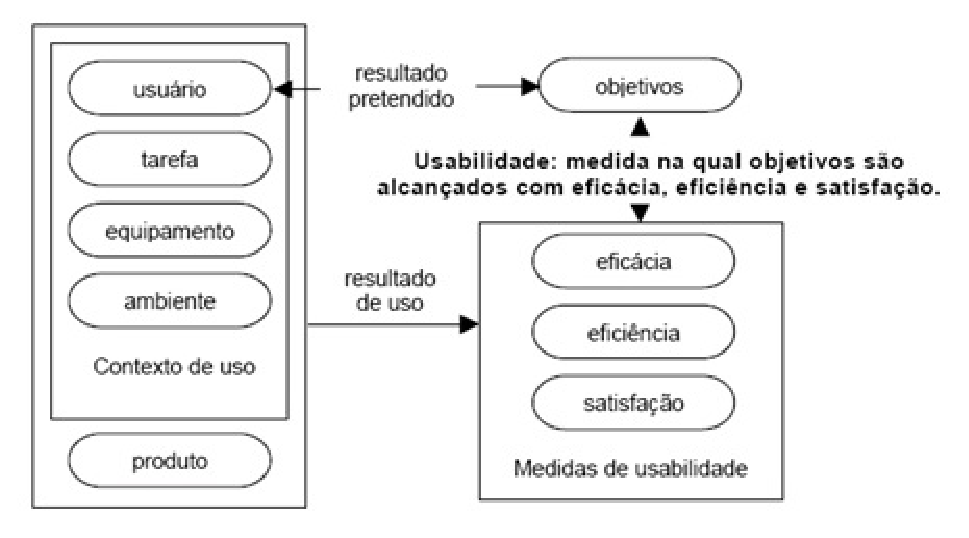
\includegraphics[keepaspectratio=true,scale=0.60]
      {figuras/estruturausabilidade9241.eps}
    \caption{Estrutura de Usabilidade Norma ISO 9241-11}
    \label{estrutura_usabilidade}
\end{figure}

\subsection{Metas de Usabilidade}

	As metas de usabilidade servem para guiar o desenvolvimento de produtos fáceis de usar, eficientes e agradáveis ~\cite{preece2007}. São elas:

\begin{enumerate}
\item Utilidade
\item Eficácia
\item Eficiência
\item Segurança
\item Facilidade de aprendizado
\item Facilidade de lembrar como se usa
\end{enumerate}

% escrever mais detalhes ou inserir em outro lugar.

\section{As áreas da Usabilidade}

	Para entender o que é usabilidade e como ela está inserida no ciclo de vida do desenvolvimento de software precisamos compreender as relações que o termo tem com as diversas áreas que a envolve. 

\subsection{Interação Humano Computador}

	O Termo Human Computer Interaction  (HCI) começou a ser adotado na década de 1980 para descrever uma nova área de estudo na qual se preocupavam em saber como o uso dos computadores poderia enriquecer a vida pessoal e profissional dos seus usuários ~\cite{moraes2002}.
 
	A interação humano computador tem o principal objetivo de melhorar a eficácia e proporcionar satisfação do usuário.O objetivo do HCI são desenvolver e aprimorar sistemas computacionais nos quais os usuários possam executar tarefas com segurança, eficiência e satisfação ~\cite{preece2007}.
	
\subsection{Arquitetura da Informação}

A informação é algo que está presente no nosso dia-a-dia. Para ~\cite{wurman1991}) a informação deve ser aquilo que leva à compreensão. A quantidade de conteúdo que é produzido na internet extrapola a capacidade humana de retenção da informação. Para ~\citeonline{agner2004}, esse excesso de informação contribui para o aumento dos problemas de usabilidade e da necessidade de pesquisa na área de interação humano-computador.

Segundo ~\citeonline{garret2003}, a arquitetura da informação são a arte e a ciência de estruturar e organizar os ambientes informacionais para ajudar as pessoas a encontrarem e administrarem informações.

O arquiteto de informação deve ser um profissional multidisciplinar com conhecimentos em design gráfico, ciência da informação, biblioteconomia, jornalismo, engenharia de usabilidade, marketing e ciência da computação. Ele deve balancear as necessidades do usuário com os objetivos do negócio ~\cite{rosenfeld1998}.

\subsection{Ergonomia}

A ergonomia está na origem da usabilidade, pois visa proporcionar eficácia e eficiência, além de bem-estar e saúde do usuário através da adaptação do trabalho ao homem. O seu objetivo é garantir que sistemas e dispositivos estejam adaptados às maneiras de pensar, agir e trabalhar do usuário. ~\cite{cybis2010} 

\subsection{Design Centrado no usuário}

	Design centrado no usuário é um campo de estudo que reúne metodologias de design nas quais o público álvo de um produto ou serviço influencia as diretrizes e requisitos do sistema ~\cite{norman2006design}.
	
	Para ~\citeonline{norman2006design}, cunhador do termo, o design centrado no usuário é uma filosofia baseada nas necessidades e interesses dos usuário, com ênfase em fazer produtos úsaveis e inteligíveis. 

	Segundo ~\citeonline{saffer2010designing} as pessoas que utilizarão um produto ou serviço sabem de suas necessidades, metas e preferências, e é papel do design descobrir isto e projetar para eles e essa é a filosofia por trás do design centrado no usuário.

\subsection{Design de Interaçao}

	Uma grande parte dos produtos que necessitam da interação do usuário são feitos olhando apenas na perspectiva da engenharia e se esquecem de seus reais usuários. O design de interação surge para redirecionar a preocupação que se tinha apenas em produzir algo que funcionasse para produzir algo que sejá fácil de utilizar, agrádavel e eficaz na perspectiva do usuário, trazendo a usabilidade para dentro do processo de design ~\cite{preece2007}.

	Segundo ~\citeonline{moggridge2006}, o termo surgiu com Bill Verplank que resume design de interação a partir da resposta de três perguntas sobre como você age, como você sente e como você compreende. 
	
	Uma outra definição de design de interação é o design de produtos interativos que fornecem suporte à atividades cotidianas das pessoas, seja no lar ou no trabalho, ou seja, criar experiências que melhorem, estendem a maneira como as pessoas trabalham, se comunicam e interagem ~\cite{preece2007}.

	
\subsection{Engenharia de Usabilidade}

A engenharia de usabilidade surgiu no final dos anos 80 com o esforço sistemático das empresas e organizações para desenvolver programas de software interativo com usabilidade. Sua origem parte de iniciativas de cientistas como Card, Moran e Newell (Modelo do processador Humano de 1983) e Norman (Teoria da Ação de 1989). O objetivo era produzir conhecimentos que favorecesse a concepção de interfaces humano-computador mais adaptadas ~\cite{cybis2010}.

Podemos fazer um paralelo da engenharia de usabilidade com a engenharia de software. A engenharia de software ocupa do desenvolvimento do núcleo funcional de um sistema interativo formado por estruturas de dados, algoritmos e recursos de processamento de dados. Esse núcleo é construído de forma que o sistema funcione bem, de forma correta, rápida e sem erros. Já a engenharia de usabilidade ocupa-se da interface com o usuário que interliga as funções do sistema com os usuários de forma que a interface do sistema seja agradável, intuitivo, eficiente e fácil de operar ~\cite{cybis2010}.



\subsubsection{Ciclo de Engenharia de Usabilidade}

	O ciclo foi definido sendo essencialmente evolutivo, interativo e baseado no envolvimento do usuário. A norma ISO 13407 (Projeto centrado no usuário) sugere quatro principais etapas desse ciclo (analisar e especificar o contexto de operação; especificar as exigências dos usuários e organizações; produzir soluções de projeto; avaliar o projeto contra as exigências) ~\cite{cybis2010}.

\subsection{Experiência do Usuário - UX}

	Experiência do usuário é toda a interação com um produto, serviço ou marca. O termo é usado frequentemente para sintetizar toda a experiência com um produto de software. Não engloba  somente as funcionalidades e sim o quanto o aplicativo é  agradável ao usuário~\cite{travis2013}.
	
	O termo User Experience (UX) foi cunhado por Donald Norman na década de 80 para cobrir todos os aspectos da experiência da pessoa com o sistema. Acreditava que as definições de interface do usuário e usabilidade limitava o entendimento sobre o que o trabalho dele representava. Ele disse atualmente que não gosta do termo pois está sendo utilizado para resumir tudo o que ele estava fugindo, que é pensar em UX como apenas as disciplinas.UX não é uma disciplina é uma cultura. \footnote{\url{uxdesign.blog.br}}

	Qualquer pessoa envolvida no projeto precisa atuar na experiência do usuário e deve ser feito em todo o processo.


\subsection{Relação de todas essas áreas com a Usabilidade}

	A usabilidade está relacionada com os fatores humanos e corresponde como o estudo de como usuários se relacionam com qualquer produto. A interação humano computador está baseada na usabilidade e foca no modo como as pessoas se relacionam com os produtos ligados à computação.

	As áreas que trabalham com usabilidade são disciplinas transversais que agregam diversas áreas do conhecimento tais como pscicologia, sociologia, ciência da informação e da computação, fatores humanos, design gráfico e indústrial, ergonomia, comunicação e etc.

 
%------------------------------------------------------------------------------%

\section{A importância e os benefícios da Usabilidade}

No modo geral, os projetistas sabem da importância de desenvolver com enfoque no usuário e na usabilidade, mas normalmente os projetos são desenvolvidos sem que tenham sido realizadas pesquisas e aplicados métodos e técnicas de usabilidade.
	
	O tempo e os recursos limitados são as principais razões que impede a implatação dos testes de usabilidade nas equipes de software. Também há o desconhecimento por parte da equipe de desenvolvimento das técnicas a serem empregadas.

	Segundo ~\citeonline{rosa2012}, incorporar a usabilidade no seu processo pode reduzir os custos e tempo de desenvolvimento e melhorar o produto final. É preciso ter em mente quem é o seu usuário final em todas as etapas de desenvolvimento e processos de produção, desde análise das necessidades e projeto conceitual até prototipagem e produção. 

	O investimento na área de usabilidade agrega valor ao produto e traz benefícios não somente aos usuários, mas também aos seus produtores. 

	Para a Associação de Profissionais de usabilidade (UPA), a usabilidade inclui os seguintes benefícios:

\begin{itemize}
\item Aumentar a produtividade
\item Diminuir custos de treinamento e suporte
\item Aumentar as vendas e as revendas
\item Reduzir os custos de desenvolvimento e manutenção.
\item Aumentar a satisfação do consumidor.
\end{itemize}


%------------------------------------------------------------------------------%. 

\section {Avaliação de Usabilidade}

	
	Os métodos de avaliação são utilizados para avaliar a qualidade das interações entre o usuário e o sistema, e para verificar, inspecionar e diagnosticar os aspectos ergonômicos das interfaces.

	As avaliações de interface podem ser divididas de diversas maneiras como o tipo de dados, formas e o local da avaliação. Quanto a forma, pode ser definida como:

	\begin{itemize}
		\item \textbf{Objetiva:} São baseadas em técnicas que utilizam medições quantitativas, em vez de opiniões dos usuários ou especialistas.
		\item \textbf{Subjetiva} São baseadas em opiniões e relatos de usuários e especialisatas.
	\end{itemize}

	Quanto ao tipo de dados, pode ser definida como:

	\begin{itemize}
		\item \textbf{Quantitativa} Envolvem medidas e tendem a ser vistas como objtivas e imparciais.
		\item \textbf{Qualitativa} Envolvem descrições e relatos e são vistas como subjetivas.
	\end{itemize}

	Quanto ao local da avaliação:

	\begin{itemize}
		\item \textbf{Laboratório} Ocorre em ambientes controlados.
		\item \textbf{Estudo de Campo ou natural} Estão situados no contexto do mundo real no qual o sistema é utilizado.
	\end{itemize}

	 
	Antes de definir as técnicas de avaliação ~\citeonline{preece2007} identifica quatro tipos de paradigmas de avaliação: (1) avaliações rápidas e sujas; (2) testes de usabilidade; (3) estudos de campos e; (4) avaliações preditivas.

	Em relação as técnicas de avaliação, ~\citeonline{preece2007} as divide em cinco técnicas de avaliação: (1) observação e monitoramento; (2) opinião dos usuários; (3) opiniões dos especialistas; (4) testes com os usuários e; (5) Predição. 

	Já ~\citeonline{cybis2010} divide as técnicas de avaliação da usabilidade de interfaces em três grupos. Técnicas prospectivas; técnicas preditivas/diagnósticas/analíticas/inspecção e as objetivas/definitivas/empíricas.

	De acordo com ~\citeonline{preece2007} cada método de avaliação possui características e pode ser aplicado em diferentes situações. Eles diferem entre si em vários aspectos. É preciso entender as diferentes caracterśiticas de cada método para se definir qual deles é o mais apropriado para avaliar a interface de um software em um determinado contexto. Cada método pode se diferenciar pela etapa do ciclo que pode ser aplicado, a técnica utilizada para coletar dados e os tipos de dados coletados (quantitativa ou qualitativa). 

\section{Técnicas e Métodos da Engenharia de Usabilidade}

	Esta seção mostra as técnicas e os métodos que são utilizados pela interação humano computador para desenvolver um sistema com usabilidade.

	De acordo com ~\citeonline{bervian2002metodologia} as técnicas são procedimentos específicos utilizados por uma ciência determinada. O conjunto com várias técnicas constituem os métodos. Algumas técnicas são utilizadas em várias ciências e os métodos se adapta às diversas ciências a medida que há imposição de uso de técnicas especializadas.

	~\citeonline{cybis2010} divide as técnicas e os métodos da engenharia de usabilidade em três tipos: Concepção, Análise e Avaliação.

\subsection{Métodos e técnicas de concepção}

	Os métodos de concepção são utilizados para implementar as especificações e os requisitos para a interface a usabilidade de um sistema.

\subsubsection{Brainstorming}

	O brainstorming é bastante utilizado em ambientes ágeis para obter ideias, entrar em consenso sobre problemas ou novas propostas.

\subsubsection{Storyboard}

É uma representação das interações entre os usuários e o sistema em seu ambiente de trabalho. Corresponde ao detalhamento de um cenário de uso especificado para o sistema consistindo em uma sequência de desenhos representando não só os esboços de telas, mas também os elementos do contexto (usuários, equipamentos, móveis, telefones, colegas).

\subsubsection{Card Sorting}

	É uma técnica usada para descobrir como o usuário classifica determinada informação em sua mente. O usuário recebe uma série de cartões embaralhados descrevendo conteúdos e agrupam os cartões que tenham alguma relação. Podem ser distribuidos cartões com nomes de categorias.
	

	O \textit{card sorting} pode ser aberto ou fechado podendo ser aplicado tanto de forma presencial ou remota e aplicados para grupos ou para uma única pessoa. Recomenda-se no mínimo 15 testes e que cada teste tenha 2 pessoas.
	
\subsubsection{Diagramas de Afinidade}

	Os diagramas de afinidade são utilizados para organizar uma grande quantidade de itens em grupos lógicos. Diferente do \textit{card sorting}, nesta técnica os projetistas e usuários trabalham juntos para obter consenso sobre a organização dos itens. Essa técnica pode ser usada para analisar os resultados de estudos de campo e analisar as conclusões de uma avaliação de usabilidade.

\subsubsection{Protótipos}

	Os protótipos de papel são úteis para detectar problemas de usabilidade logo no início do proceso de design. São usados para esclarecer os requisitos específicos para o projeto da interface do sistema. São rápidos de construir, permitindo rápidas interações de projeto e necessitam de poucos recursos para serem criados. 
	Existem também os protótipos de baixa, média e alta que simulam o sistema com mais fidelidade do que os protótipos em papel. 

%------------------------------------------------------------%%%

\subsection{Métodos e técnicas de análise}

Estes métodos são utilizados para buscar informações sobre o contexto de uso e sobre a usabilidade de um sistema. Podem ser feitas análises do perfil do usuário, o ambiente de uso, as tarefas, possibilidades e restrições do sistema.

As técnicas mencionadas à baixo visam apoiar os projetistas de interface na busca de informações sobre o contexto de uso e sobre a usabilidade de um sistema existente. Essas técnicas são empregadas de forma que se complementem-se umas as outras.

\subsubsection{Observação}

	Essa técnica caracteriza-se por um pesquisador observando o usuário e tomando notas, enquanto este trabalha em seu contexto usual. é uma técnica útil para obter dados quantitativos (tempo para as tarefas) e qualitativos (práticas e estratégias do usuário) ~\cite{cybis2010}.

	No planejamento é importante definir os objetivos e as maneiras de como será registrada os acontecimentos. Deve-se levar em consideração o fato que muitos usuários por estarem sendo observados podem alterar seu comportamento ao utilizar a ferramenta. É importante que todos estejam cientes dos objetivos do estudo, deixando claro que não é ele que será avaliado e sim conhecer uma situação de uso.

\subsubsection{Entrevistas Tradicionais}

Através de entrevistas podemos obter as opiniões tanto dos usuários atuais como dos futuros usuários dos sistemas. Primeiramente é importante identificar as necessidades das pessoas em acessar uma determinada informação.

\subsubsection{Eyetracking}

Eyetracking é uma técnica que rastrea o movimento dos olhos e da cabeça para registrar a tomada de informações numa interface.

\subsubsection{Questionários de Perfil de Uso}
 
É utilizado para obter informações sobre as caracteristicas reais dos usuários de um sistema e saber como eles realmente utilizam tais ferramentas. É importante que ao utlizar os questionários de perfil de uso é preciso definir um foco para a sua pesquisa. Deve-se identificar as principais dúvidas da equipe de projeto em relação ao uso do sistema ~\cite{cybis2010}.

Este tipo de questionário pode ser enviado para os emails dos usuários da ferramenta em análise. É importante definir o tamanho de sua amostra. De acordo com ~\citeonline{cybis2010}, de 20 a 30 por cento é a taxa de retorno dos questionários enviados. As respostas podem ser analisadas utilizando métodos estatísticos.


\subsubsection{Questionários de Satisfação}

	A aplicação de questionários é um dos métodos mais utilizados para avaliação da satisfação do usuário. Eles resultam da avaliação subjetiva pelo usuário, o qual é influenciado pelos tipos de questões aplicadas.
	
	Questionários de satifação são utilizados principalmente quando existem usuários experientes que utilizam o sistema com frequência, podendo ter informações fidedigna sobre aspectos satisfatórios e insatisfatórios no sistema. Também podem ser aplicados por usuários de uma nova versão de um sistema imediatamente após um teste de usabilidade. Essa relação com os testes de usabilidade é interessante por permitir a correlação das medidas de desempenho (tempo, frequência) com as medidas de satifação do usuário ~\cite{cybis2010}.

	É recomendado que se utilize um questionário padronizado, pois permite a comparação de resultados obtidos por diferentes sistemas. Estes questionários apresentam opções de respostas fechadas, o que permite a produção de dados quantitativos e objetivos ~\cite{cybis2010}.

	Um grande número de questionários foram desenvolvidos pela comunidade científica para a avaliação da usabilidade.  Alguns exemplos de questionários são: QUIS, SUMI,  WAMMI, SUS, ASQ, PSQ,PSSUQ, CSUQ. Os detalhes referentes a cada questionário estão detalhados no apêndice.

\subsubsection{Grupos de Foco}

	Grupo focal é uma reunião informal de usuários que manifestam suas opiniões sobre o determinado assunto, que pode ser tanto uma oportunidade de novas uncionalidades ou algum problema específico.

	Um moderador deve preparar um roteiro  com uma lista de assuntos a serem tratados. É importantes que os participantes sejam de perfis diferentes para que possa ter uma maior diversidade de informações. Costuma-se ter em média de 6 a 12 usuários em uma mesa de reuniões. Os registros das informações podem ser através de vídeos ou blocos de anotações. O objetivo não é ter a obtenção do consenso em torno das ideias, mas sim ter uma boa quantidade de opiniões sobre o assunto a ser tratados ~\cite{cybis2010}.


\subsubsection{Diários}

	É uma técnica útil quando a experiência do usuário é ampla e depende da utilização em multi lugares. Nessa técnica os usários carregam consigo um pequeno diário para nele anotar as informações do seu dia-a-dia na utilização do sistema ~\cite{cybis2010}.

\subsubsection{Benchmarking de Usabilidade}

	Benchmarking é definido como método sistemático e contínuo de avaliação de sistemas reconhecidos como representantes das melhores e mais eficazes pŕaticas com a finalidade de comparar desempenhos e identificar oportunidades de melhoria. ~\cite{spendolini1994}

	Este método parte da definição dos critérios de avaliação e seleção de representantes relevantes para criar uma listagem de caracterśisticas desejáveis para o futuro sistema, como também os aspectos que são desfavoráveis e que devem ser evitados.

\subsubsection{Cenários de uso}

	É uma técnica simples e eficaz para analisar e comunicar uma parte das especificações de requisitos produzidos para a usabilidade e a interface. São utilizados para comunicar os cenários atuais de uma tarefa (problema) e o cenário futuro (solução). Os cenários de solução deve descrever em linguagem natural, como determinados usuários realizarão tarefas específicas com o sistema em um determinado contexto. É preciso decompor os objetivos dos usuários segundo as operações necessárias para alcança-los, identificando as atividades que serão realizadas pelos usuários ~\cite{cybis2010}.

\subsubsection{Personas}

	A técnica de persona descreve o perfil de uma pessoa fictícia envolvida com o produto. Trata-se de inventar um conjunto de pessoas (três ou quatro) que estejam dentro da população de usuários pretendidos e descrevê-las em detalhes ~\cite{cybis2010}.

	As informações devem ser qualitativas e coletadas por meio de entrevistas e questionários junto à população alvo do sistema. As personas permitem maiior entendimento dos usuários, colocando-os no centro das decisões do projeto ~\cite{cybis2010}. Essa técnica tem objetivos similares aos de cenários, porém ao invês do foco ser na tarefa, deve-se ter foco em uma pessoa que faça parte do público alvo do sistema.


\subsection{Técnicas e Métodos de avaliação}


\subsubsection{Checklists}

	\textit{Checklist} é uma técnica de inspeção qu oferece uma maneira de abordagem rápida, fácil e de baixo custo para a avaliação de uma interface. Permite com que usuários que não são especialistas em ergonomia identificarem problemas menores e repetitivos.~\cite{cybis2010} 

	Várias vantagens são encontradas na utilização dessa técnica como: redução de custos de avaliação por não precisar de especialistas; sistematização das avaliações; reduz a subjetividade dos processos de avaliação e fornece um conhecimento ergonômico sobre o que avaliar.

	O Ergolist \footnote{\url{http://www.labiutil.inf.ufsc.br/ergolist/check.htm}} é um aplicativo que pode ser utilizado para realizar uma inspeção da qualidade ergonômica da interface com o usuário do sistema.

\subsubsection{Avaliação heurística}

	Representa um julgamento de valor sobre as qualidades ergonômicas das interfaces Humano-Computador. Essa avaliação é realizada por especialistas em ergonomia e usabilidade. Eles examinam o sistema interativo e diagnosticam os problemas ou as barreiras que os usuários provavelmente encontrarão durante a interação ~\cite{cybis2010}.

	O principal objetivo desse tipo de avaliação é avaliar a interface em fases iniciais do sistema, sem o envolvimento do usuário. Os graves problemas de interface devem ser localizados antes que realizem os testes de usabilidade com usuários reais ~\cite{santos2012}.

	As avaliações mais utilizadas são as 10 heurísticas de ~\citeonline{nielsen1994}. São elas:

	\begin{itemize}
		\item{Visibilidade de acordo com o sistema}
		\item{Mapeamento entre o sistema e o mundo real}
		\item{Liberdade e controle ao usuário}
		\item{Consistência e Padrões}
		\item{Prevenção de Erros}
		\item{Reconhecer em vez de relembrar}
		\item{Flexibilidade e Eficiência de uso}
		\item{Design estético e minimalista}
		\item{Suporte para usuário reconhecer, diagnosticar e recuperar erros}
		\item{Ajuda e documentação}
	\end{itemize}


	Pesquisas realizadas por Jakob Nielsen fornecem indicações sobre a quantidade de avaliadores que devem ser consultados para que possam indentificar grande parte dos problemas de ergonomia. Cinco avaliadores com experiência tanto em usabilidade como no sistema consegue identificar 95 por cento dos problemas de ergonomia enquanto especialistas que conhece apenas de usabilidade identificam 85 por cento.

\begin{figure}[h]
    \centering
    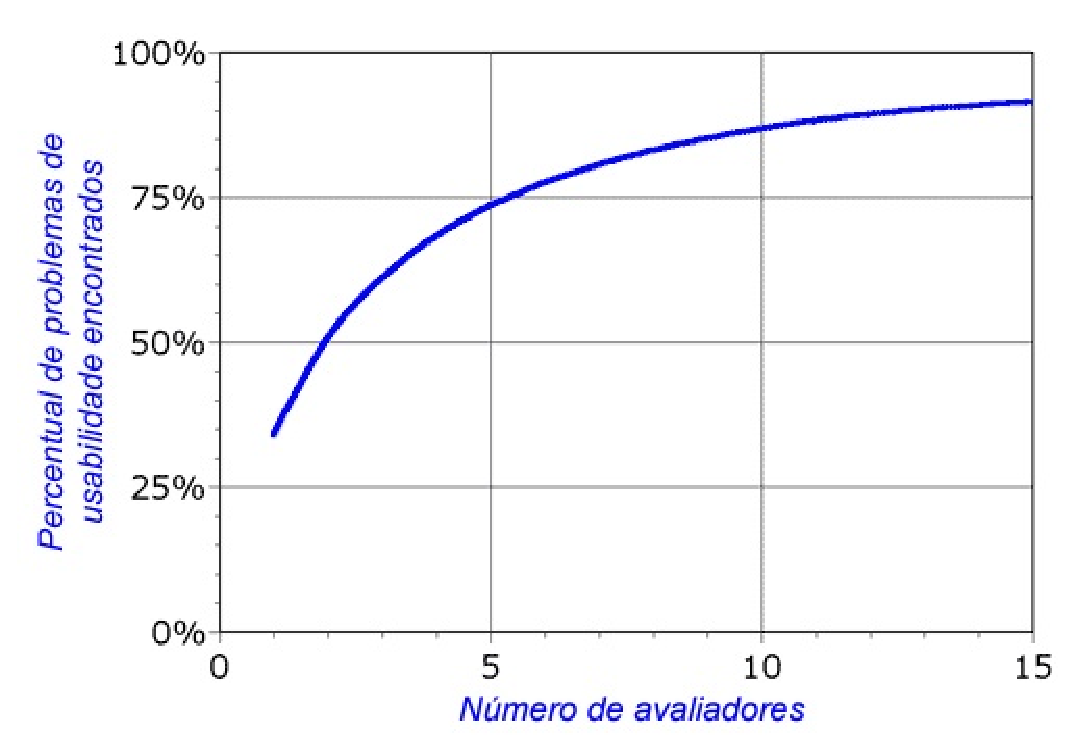
\includegraphics[keepaspectratio=true,scale=0.60]
      {figuras/avaliadores_heuristica.eps}
    \caption{Número de avaliadores~\cite{nielsen1994}}
    \label{avaliadores}
\end{figure}

	A avaliação heurística requer pouco planejamento e pode fazer parte de um processo interativo de um projeto e aplicado em todas as fases de desenvolvimento da interface, mas é preciso que seja avaliado por especialistas de usabilidade com pleno conhecimento nas heurśiticas.
	

\subsubsection{Listas de Verificação}

	Permitem que profissionais que não necessariamente sejam especialistas em ergonomia identifiquem problemas menores e repetitivos das interfaces. As normas ISO 9241, partes 10 a 17, fornecem listas de verificação de ergonomia bem definidas, assim como as fornecidas pelo site Ergolist ~\cite{cybis2010}.
	

\subsubsection{Percurso Cognitivo}

Percurso cognitivo é um método de inspeção de usabilidade que tem como objetivo avaliar a interface considerando a facilidade da interface. A finalidade do percurso cognitivo é fazer com que o design de interação seja fácil de aprender por meio da exploração. Os inspetores aplicam uma lista de verificação orientada à tarefa interativa, abordando os processos cognitivos que se estabelecem quando o usuário a realiza pela primeira vez ~\cite{cybis2010}


\subsubsection{Teste de Usabilidade}

	É um dos métodos de teste de experiência do usuário (UX) mais frequentemente utilizado e conhecido entre aqueles que não são projetistas da UX. Realizar testes com usuários é o núcleo do Design Centrado no Usuário, pois é através destes que podemos saber se as reais expectativas dos usuários são atendidas ~\cite{santos2012}.

	O teste consiste em avaliar o desempenho dos usuários na execução de tarefas cuidadosamente preparadas, tarefas estas dentro do escopo do sistema. Esse desempenho pode ser avaliado no quesito, número de erros e tempo de execução da tarefa, questionários e entrevistas também podem ser utilizados. ~\cite{preece2007}

	Existe alguns passos comuns que devem ser seguidos para a execução dos testes de usabilidade:

\begin{itemize}

\item \textbf{Escolher abordagem}

	Existem vários tipos de testes de usabilidade, mas sabe-se que todos eles têm algo em comum, que é observar as pessoas utilizando algo.As abordagens de pesquisa podem ser de dois tipos: quantitativa ou qualitativas. 

	Pesquisas quantitativas são focadas nos dados numéricos e é voltada para fornecer alta confiança e resultados repetidos dentro de seus grupos de usuários.É preciso ter o envolvimento de um número maior de participantes para contar as variações que você encontrará de indivíduo para indíviduo ~\cite{unger2009}.

	Os testes quantitativos são como experimentos cientificos que precisam ser rigorosos ou os resultados não serão confiáveis. Deve-se definir um protocolo de teste e segui-lo consistentemente para todos os participantes ~\cite{krug2010}.

	As pesquisas qualitativas não são focadas em níveis de segurança e da possibilidade de repetição, mas sim ganhar contexto e percepção considerando o comportamento do usuário.Ela depende da interpretação do projetista sobre as descobertas, a intuição e o senso comum ~\cite{unger2009}.

	Nos testes qualitativos você tenta minimizar a quantidade de interação com o participante para evitar a influência nos resultados ~\cite{krug2010}.

	Para os testes de usabilidade é possível utilizar qualquer uma das abordagens, mas a qualitativa é a mais acessível para aqueles que não tiveram um treinamento em métodos científicos mais formais e oferece uma rica fonte de dados ~\cite{unger2009}.



\item \textbf{Planejar a pesquisa}

Algumas questões devem ser respondidas ao criar o teste de usabilidade: Estas questões te ajudam a oferecer foco e escopo. Abaixo algumas perguntas que devem ser respondidas no planejamento de sua pesquisa:

\begin{itemize}
\item Defina seu objetivo: Por que você está testando? %Cap2
\item Defina Usuários: Quem você está testando? %Cap6e7
\item Defina o método para representar sua aplicação: O que você está testando?
\item Quais informações você está reunindo? 
\end{itemize}

Nas pesquisas qualitativas geralmente queremos compreender as questões que os usuários podem encontrar, os níveis de frustações que eles podem experimentar e a gravidade de um problema em particular. Para os testes qualitativos devem se pensar em medidas que serão possíveis de ser respondidas com cinco usuários ~\cite{unger2009}. 

	\begin{itemize}
		\item Taxa de Sucesso: O grau em que o usuário foi capaz de completar a tarefa?
		%Pode-se detalhar com mais informações sobre o que seria a taxa de sucesso, e o que é considerado o sucesso.
		\item Satisfação do usuário
	\end{itemize}

\item \textbf{Usuários}

Existem algumas diretrizes que podem ser adotadas para a definição da quantidade de usuários. ~\citeonline{nielsen1994} definiu algumas dessas diretrizes:

\begin{itemize}
\item No teste quantitativo planeje uma quantidade maior de participantes. Em média 20 por rodada de pesquisa.
\item No teste qualitativo é suficiente ter entre 5 e 8 participantes.
\end{itemize}

	 ~\citeonline{krug2010} defende a ideia de que três usuários são ideais para realização de testes de usabilidade para quem está realizando o teste por conta própria. Ele afirma que é mais fácil encontrar três participantes do que uma quantidade maior e que é bem provável que eles já encontrem muitos dos problemas significaticos relacionados as tarefas que você está testando.

	Em equipes ágeis, o teste com o usuário é realizado com o cliente do projeto e envolve o especialista em usabilidade como mediador do teste ~\cite{santos2012}.

\item \textbf{Recutramento e logística}

Depois de ter feito o plano de pesquisa e definido os tipos de usuários que podem ser inseridos na pesquisa é hora de recrutar os participantes.
Para o recrutamento de participantes é interessante gerar uma lista com os potenciais participantes do teste. Essa lista pode vir de usuários registrados do site da empresa relacionada; informações de contatos do cliente; e-mails para conhecidos que tenha relação com o assunto do teste; requisições em pequenas pesquisas que pré-qualificam os participantes, e etc.~\cite{unger2009}.

Você pode realizar uma filtragem com os participantes potenciais antes de seleciona-los. As perguntas do questionário de filtragem devem ser voltadas para:

	\begin{itemize}
	\item Garantir que o participante seja um usuário das funções em que você está testando.
	\item Determinar se ele se encaixa em um dos seus grupos de usuários.
	\item Ajudar a ter uma boa mistura de participantes.
	\end{itemize}

O questionário de perfil de usuário pode ser utilizado para realizar essa filtragem de participantes.


\item \textbf{Criação de guias de discussão}

Para a execução do teste de usabilidade é preciso que as instruções estejem claras aos participantes, contendo todas as informações específicas que ele precisará para completar as tarefas com sucesso.

Os seus materiais de teste deve incluir:

	\begin{itemize}
		\item Formulário de consentimento para gravação de vídeo
		\item Guia de discussão para o participante, com tarefas detalhadas e perguntas sobre a satisfação do usuário.
		\item Questionários
	\end{itemize}

\item \textbf{Facilitação}

\item Análise e apresentação dos resultados;
\item Criação de recomendações.

\end{itemize}


%------------------------------------------------------------%

\section {Usabilidade em Software Livre}

	Um dos grandes problemas encontrados em softwares livres é a pouca atenção dada aos aspectos referentes a usabilidade e acessibilidade das aplicações. Acredita-se que um dos principais problemas que contribui para a falta de usabilidade de software livre é sua própria comunidade que apenas enfatiza na criação e, melhoria e teste do código fonte.  

Segundo ~\citeonline{preece2007}, uma das causas da baixa adoção de softwares livres em mercados de larga escala é a baixa qualidade dos estilos de interação implementados nas interfaces dos produtos. Uma grande maioria não se preocupa com bons elementos de interface com usuário (UI). 

Atualmente, algumas comunidades de software livre vêm se atentando as questões de usabilidade como forma de se manter no mercado. Um dos casos que conhecemos foi do Joomla que é um sistema de gerenciamento de conteúdo  que nessas últimas versões investiram em questões de usabilidade, sendo o primeiro CMS a ser totalmente responsivo. Foi criada uma frente de desenvolvimento focado na experência do usuário que trouxe melhorias significativas a partir da versão 3.0 do CMS. Logo em seguida o Wordpress, outro sistema de gerenciamento de contéudo investiu em melhorias da interface se atentando aos novos padrões adotados na web.

	Uma grande dificuldade encontrada por parte de usuários com pouca experiência se encontra na instalação de softwares livres o que acaba por desencorajar esses usuários na utilização desses softwares.
	
Entender o perfil do usuário é um dos principais pontos que devem ser levados em consideração pelos desenvolvedores de software em geral. Cada perfil de usuário tem suas particularidades e suas expectativas quanto a utilização do sistema. Quando falamos de usuários com experiência de uso de softwares semelhantes é preciso ter uma maior atenção na usabilidade para que possa ter uma boa aceitação e menor impacto com as mudanças.



%---------------------------------------------------------%

\section{Processos de Usabilidade}


	Alguns autores como ~\citeonline{mayhew1999} e ~\citeonline{hix1993} proposeram modelos de processo baseados em ciclo de vidas bem definidos para as atividades de usabilidade.Outro modelo muito utilizado para descrever processos de usabilidade é o proposto pela norma ISO/IEC-13407 (1999).

	O termo modelo de ciclo de vida é utilizado para representar um modelo que capta um conjunto de atividades e a maneira como elas se relacionam ~\cite{preece2007}.

\subsection{Modelo Estrela}

	Proposto em 1989 por ~\citeauthor{hix1993}, o modelo de ciclo de vida estrela derivou do trabalho empírico de entender como os designers lidavam com os problemas de design em IHC. Eles observaram dois diferentes modelos de trabalho: analítico e o sintético. O primeiro parte-se da visão do sistema para a visão do usuário, já o segundo da visão do usuário para a do sistema ~\cite{cybis2010}.

	No modelo estrela não há especificação de ordenamento de atividades. Pode-se ir de uma atividade à outra há qualquer momento, desde que passe primeiramente pela avaliação. Sempre que uma atividade for completada deve-se avaliar o seus resultados.

\begin{figure}[h]
    \centering
    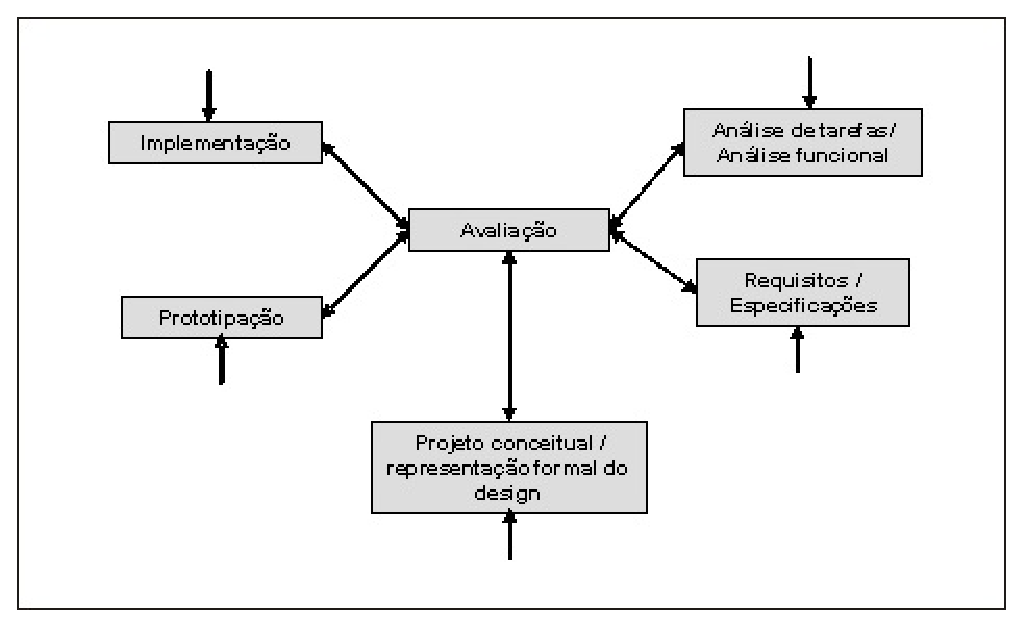
\includegraphics[keepaspectratio=true,scale=0.60]
      {figuras/estrela.eps}
    \caption{Ciclo de Vida Estrela}
    \label{ciclo_estrela}
\end{figure}

\subsection{O ciclo de vida da Engenharia de Usabilidade - Mayhew}

	O ciclo proposto por ~\citeonline{mayhew1999} oferece uma visão holística acerca dessa engenharia e uma descrição detalhada de como podemos realizar os testes de usabilidade.% ~\cite{preece2005}.

	A primeira etapa do ciclo é a análise dos requisitos. Mayhew propõe quatro tipos de atividades de análise de requisitos que são detalhadas abaixo:

\begin{itemize}
\item \textbf{Análise do perfil do usuário:} Os projetistas devem conhecer os atributos pessoais e suas habilidades para cada tipo de usuário identificado. 
	
\item \textbf{Análise do contexto da tarefa:} Os projetistas devem conhecer os objetivos e resultados, a estrutura, duração, custos e etc. de cada tarefa a ser realizada.

\item \textbf{Análise das possibilidades e restrições da plataforma:} Verificar quais são as possibilidades e restrições em termos de equipamentos, sistems operacionais e etc.

\item \textbf{Análise dos princípios gerais para o projeto:} Atividade relacionada à pesquisa e catalogação dos conhecimentos de ergonomia disponível para a concepção da interface no tipo de contexto de uso.

\end{itemize}

	Depois da análise dos requisitos é preciso especificar as metas de usabilidade do futuro sistema. A norma ISO 9241:11 orienta como podemos especificar essas metas.

	Na etapa de projetos, testes e implementação, Mayhew propôs que os ciclos devem se repetir de forma a tratar três nivéis de aspectos de uma interface: No primeiro nível sendo a interface definida conceitualmente; no segundo nível refere-se as definições em termos de estilo; e no terceiro nível as interações e componentes relacionados com os contextos das tarefas especiais. A última fase é a de instalação do sistema onde depois que o usuário já estiver acostumado com o sistema ele pode dar um \textit{feedback} sobre a usabilidade do produto de forma mais fidedigna por já ser um "especialista" da ferramenta como cita a autora. 

	Uma das técnicas utilizadas para coletar \textit{feedback} são os testes de usabilidade no local do trabalho dos usuários ou utilizando métodos de análise como entrevistas, observações, questionários, grupos de discussões. Esses métodos serão detalhados no pŕoximo cápitulo.


\subsection{Design Centrado no Usuário}

O DCU surgiu da IHC e consiste em uma metodologia de design de software para desenvolvedores e designers. Foi definida pela norma ISO 13407 (\textit{Human Centered Design Processes for Interactive Systems}) e tem como objetivo definir um processo necessário ao desenvolvimento de produtos fáceis de utilizar na qual deve envolver os usuários no processo de desenvolvimento e na avaliação dos produtos.

Sabemos que a ciência experimental que utiliza-se dos métodos empíricos tradicionais para coletar dados e testar hipóteses sobre o comportamento humano aplicam-se de várias técnicas em nome de pessoas. Essa abordagem é preocupada com os usuários quando as representa mas ela não leva em conta diversos aspectos do usuário real, por não envolvê-los no processo. Não basta fazer para o usuário, é preciso fazer com o usuário ~\cite{eason1995}. 

No Design Centrado no usuário (DCU) diferente dos métodos empíricos tradicionais que tem o usuário apenas como  referência, no DCU o usuário tem que ser o elemento central e é necessário envolvê-lo do início ao fim do projeto. Baseia-se nas necessidades, desejos e limitações das pessoas. Deve-se iniciar com usuários e suas necessidades em vez de começar com a tecnologia. ~\citeonline{travis2013} afirma que "para criar produtos que os usuário amem, é necessário incluir os usuários no processo de criação dos produtos". 

~\citeonline{gould1985designing} estabeleceram alguns princípios para o desenvolvimento centrado no usuário na decada 70 que são utilizados até hoje que são: Foco desde o inicio nos usuários e nas tarefas, medidas empiricas e design interativo. O processo do design centrado no usuário pode ser dividido em 3 fases: análise, desenvolvimento e pós-liberação. 


\subsubsection{ISO 13407 e 9241-210}
	
A ISO 13407 define um processo geral para incluir atividades centradas em humano através do ciclo de vida de desenvolvimento sem especificar métodos exatos ~\cite{santos2012}.

A norma é caracterizada por quatro princípios: Ativo envolvimento do usuário; alocação apropriada de funções entre usuários e tecnologia; Testes de solução de design; Design multidisciplinar.Em 2010 essa ISO foi revista e renomeada para a ISO 9241-210.

Existem quatro atividades de Design Centrado no Usuário que devem estar presentes no inicío do projeto:

\begin{itemize}
\item Entender e especificar o contexto de uso;
\item Especificar os requisitos de usuário;
\item Produzir soluções de design;
\item Avaliar o design frente aos requisitos;
\end{itemize}

A ISO 13407 propõe que o envolvimento do usuário seja uma prática frequente em empresas que desenvolvem sistemas interativos.

\begin{figure}[h]
    \centering
    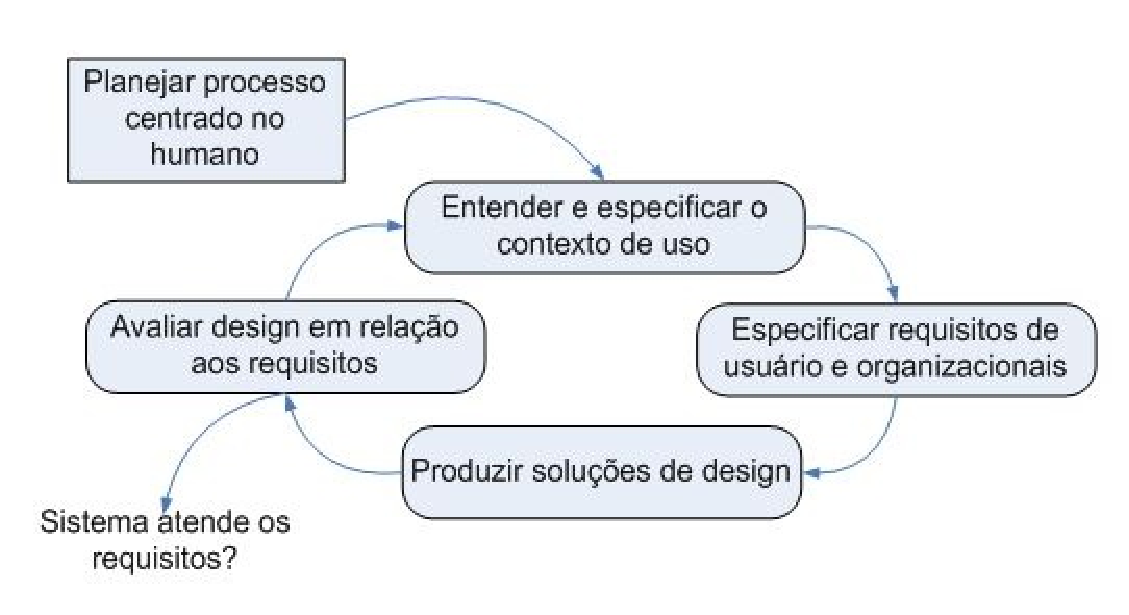
\includegraphics[keepaspectratio=true,scale=0.60]
      {figuras/ciclo_iso13407.eps}
    \caption{Ciclo do Design centrado no humano - Norma ISO 13407}
    \label{ciclo_iso13407}
\end{figure}


%------------------------------------------------------------------------------%

% Inicio da Seção sobre métodos ágeis e o design centrdo no usuário

\section{Aplicação de usabilidade em métodos ágeis}
	
	Os métodos ágeis é uma abordagem de desenvolvimento que têm como princípios um conjunto de valores com foco no cliente e nas pessoas envolvidas, na entrega constante de software funcional, no desenvolvimento iterativo baseado em ciclos curtos de entrega e na aceitação da constante mudança dos requisitos ao longo do desenvolvimento. 

	Tanto os métodos ágeis e o IHC tem esses mesmos príncipios, o que seria interessante a aplicação das técnicas utilizadas em IHC no contexto de uma abordagem ágil. Essa semelhança entre os valores proporciona um quadro favorável à integração minimalista de pŕaticas de IHC em ambientes ágeis. Podemos citar alguns desse valores como por exemplo: (i) ciclos curtos com entregas contínuas e incrementais, que favorecem a aplicação de técnicas de prototipagem; (ii) forte envolvimento do usuário que favorece a aplicação de princípios de projetos participativos e (iii) programação em pares onde em IHC geralmente a avaliação de usabilidade é feita em pares ~\cite{barbosa2008estrategia}. 

	Segundo ~\citeonline{cybis2010} as características da abordagem ágil facilitam na utilização da ergonomia e da usabilidade durante o desenvolvimento de software, mas afirma que os ergonomistas e engenheiros de usabilidade deverão adaptar suas técnicas de análise, modelagem, projeto e teste adotando-se os preceitos do manifesto ágil.
	
	As adaptações são realmente necessárias, principalmente na questão da granularidade da pesquisa, no tempo gasto com ela e na maneira de relatar as descobertas de usabilidade ~\cite{santos2012}.

	Segundo ~\citeonline{barbosa2010} é preciso ter cuidado em relação à qualidade no uso, pois raramente a comunidade ágil cita usuários ou a distinção entre usuário e cliente.

	~\citeonline{hodgetts2005experiences} afirma que os métodos ágeis são quase sempre apresentados sob a visão dos programadores, deixando de lado outras disciplinas como a UED (User Experience Design). Ele discute em seu artigo as experiências na integração de práticas do Desig da experiência do usuário em iniciativas de processos ágeis em organizações que utilizam XP e Scrum. Ele registrou os eforços da equipe com abordagem centrada apenas em métodos ágeis e depois com a integração das melhores práticas de experiência do usuário.

\subsection{Estudos correlatos}

Alguns estudos foram feitos tentando fazer essa integração da usabilidade em métodos ágeis. 

~\citeonline{constantine2002process} foi um dos primeiros a iniciar a discussão sobre o tema. Sua proposta é mostrar que UCD está prontamente integrado aos métodos ditos "leves". Ele afirma que XP e os demais métodos ágeis compartilham das mesmas fraquezas apresentadas por processos tradicionais como o processo unificado quando se refere à usabilidade e ao desenho de interface do usuário.

~\citeonline{winter2011} apresentou um estudo de caso da utilização de um pacote para teste de usabilidade que foi chamado de UIQ Technology Usability Methods (UTUM). O objetivo do estudo foi determinar como balancear as demandas de resultados ágeis e formais na execução de testes de usabilidade para garantia da qualidade.Os dados do estudo foram obtidos através da observação, entrevistas não estruturada, participações de reuniões com os stakeholders e documentos do projeto.

~\citeonline{memmel2007} mostra que é possível unir IHC e engenharia de software sob a perspectiva ágil com a utilização de um ciclo de vida de interface de usuário multidisciplinar e de Engenharia de softwre chamado CRUISER.

~\citeonline{barbosa2008estrategia} propõem uma estratégia para institucionalização da usabilidade com base em conceitos de desenvolvimento e gestão ágil. Ele realizou um workshop para reflexão sobre a importância em aplicar as novas práticas.

~\citeonline{nielsen2012} relatam um estudo na qual realizaram entrevistas com 12 especialistas em usabilidade de diferentes países no intuito de analisar a influência dos métodos ágeis nos testes de usabilidade. 

~\citeonline{lee2011} relata em seus estudos a utilização da abordagem de usabilidade ágil eXtreme Scenario-based Design (XSBD) na qual concluiram que os desafios que o time encontrava eram relacionados à comunicação, colaboração e compartilhamento de informação.

~\citeonline{wolkerstorfer2008probing} em seu estudo mostra adaptações feitas ao processo do Extreme Programming (XP). Ele integrou cinco instrumentos de IHC com o processo do XP. Os instrumentos são: testes de unidade estendidos para avaliação de usabilidade automatizada; Extreme Personas (variação do método clássico de personas); estudos de usuários para tomar conhecimento sobre o usuário final; avaliações feitas por especialistas em usabilidade e testes de usabilidade com usuários.
 
~\citeonline{leiteinspeccao}, analisou a utilização de métodos de inspeção da usabilidade no contexto de uma startup. Foi abordado duas modalidades de avaliação heuristica nessa pequan empresa de desenvolvimento de software que utiliza o método ágil Scrum. Como conclusão do estudo, relataram que a avaliação tradicional encontrou mais problemas de usabilidade e maior número de heurísticas violadas.Já na avaliação heurística colaborativa as médias de severidades atribuidas pelos avaliadores eram maior, no qual encontravam mais problemas sérios do que na avaliação tradicional, além de o tempo gasto foi menor do que na tradicional. A avaliação colaborativa apresentou características que permitia a melhor integração com ambientes ágeis.

	Outro estudo encontrado foi a proposta da metodologia AgilUS que é um método de desenvolvimento ágil que baseia-se no conceito de usabilidade e na necessidade de desenvolver software usável. Essa metodologia foi resultado de uma das linhas de investigação desenvolvida pelo Centro de Engenharia de Software da Universidade Central da Venezuela. O objetivo do método AgilUS é proporcionar um conjunto de atividades organizadas para construir a usabilidade de design de interface do usuário durante o desenvolvimento do software ~\citeauthor{acostaagilus}.

\subsection{DCU Ágil}

        Pode ser definido o DCU ágil como a prática de design centrado no usuário quando conduzida dentro de uma metodologia ou filosofia de desenvovlimento ágil de software ~\cite{santos2012}.

	O ciclo de DCU ágil foi proposto por ~\citeonline{sy2007adapting} e integra tantos as atividades de DCU como as de desenvolvimento em um único ciclo, trabalhando nas mesmas características e garantindo que as investigações de usabilidade serão tratadas durante a interação.

	Segundo \citeonline{najafi2008} o design centrado no usuário pode ser incorporado no desenvolvimento ágil sem grandes impactos no processo. No método de desenvolvimento ágil scrum, uma funcionalidade é desenvolvida, testada e documentada em uma sprint assim como no design centrado no usuário. 
	
	Segundo ~\citeonline{santos2012} o grande desafio do DCU ágil é encontrar a melhor maneira de realizar as atividades de pesquisa do usuário, design de versões que atendem as necessidades dos usuário, construção de versões interativas e realização de testes de usabilidade, dentro de um ambiente de desenvolvimento com métodos ágeis, tendo a participação dos usuários tipicos em todas as atividades.
	
        A modelagem e projeto de interfaces devem ser orientados a padrões de projeto e as avaliações de ergonomia, testes de usabilidade e especificações de revisões de interface devem ser realizados rapidamente ~\cite{cybis2010}.
	
	Pesquisas relatam que praticantes de UX que passaram a trabalhar em ambientes ágeis não querem mais retornar ao método antigo de desenvolvimento baseado no modelo cascata. Em média, essas equipes levam de 6 a 12 meses para se adptar ao novo ambiente ~\cite{santos2012}.

	O termo experiência do usuário é utilizado na comunidade ágil para qualquer atividade relacionada com a pesquisa do usuário, DCU, usabilidade, design de interfaces.A utilização do termo não indica que eles realizam todas as atividades de UX ~\cite{santos2012}.

	Segundo ~\citeonline{dickinson2010} a chave para a integração de DCU com métodos ágeis é assegurar que os resultados da pesquisa de usuário são comunicados e entendidos de forma eficaz dentro de uma equipe ágil.


\subsection {DCU e XP}

	Foram encontrados alguns estudos que descrevem a integração do IHC com as práticas de Programação Extrema (XP). Segundo ~\citeonline{mcinerney2005ucd} métodos ágeis e design centrado no usuário possuem uma cultura distinta mas eles mostraram que é possivel unir essas duas abordagens.

	O processo de usabilidade ágil é integrar os instrumentos de IHC dentro dos processos clássico de XP. ~\citeonline{wolkerstorfer2008probing} usam o dcu ágil desde 2007 e que até hoje não houve nenhum problema entre as culturas e que tanto os especialistas de usabilidade quanto os desenvolvedores estão bem integrados.Pode-se encontrar vantagens na combinação das duas abordagens. 

	Em 2008 foi proposto uma metodologia revisional institulada XPlus que insere as técnicas de design e de usabilidade em determinadas fases do ciclo de desenvolvimento de software.O XPlus agrega algumas práticas de User Experience às práticas tradicionais de XP. A figura mostra uma visão geral do processo de desenvolvimento de software de XPlus.~\cite{guimaraesxplus}

\begin{figure}[h]
    \centering
    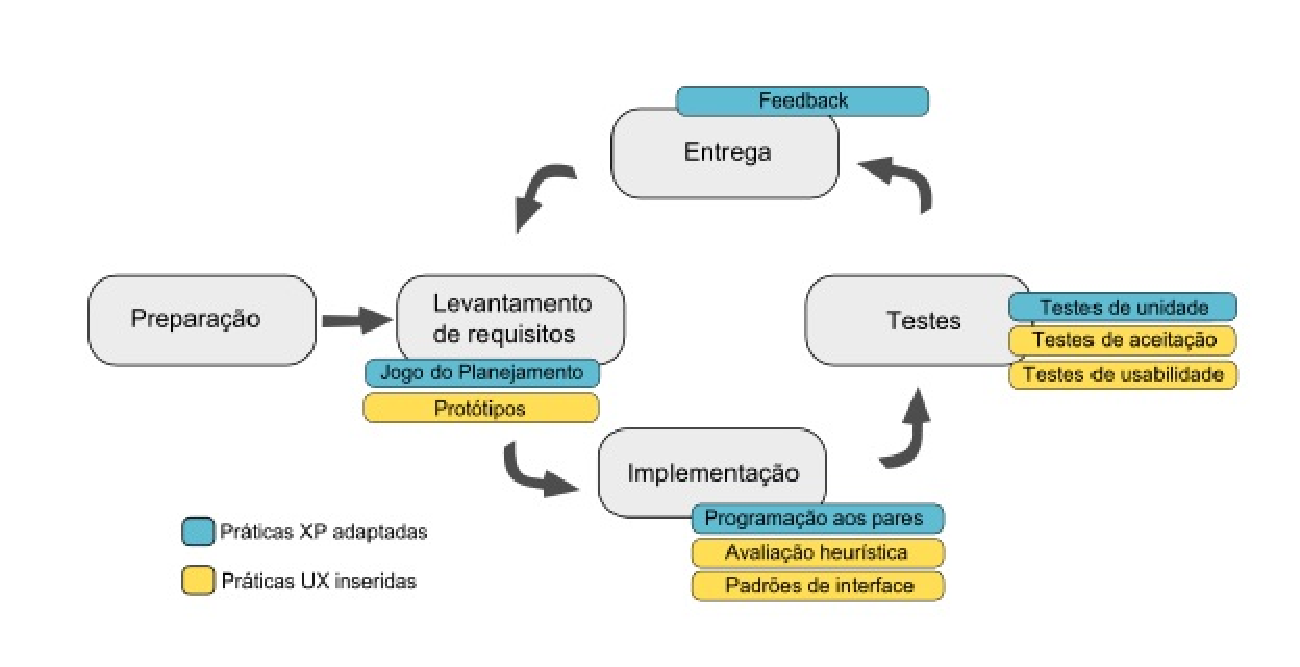
\includegraphics[keepaspectratio=true,scale=0.60]
      {figuras/xplus.eps}
    \caption{Visão geral do processo de desenvolvimento de software de XPlus}
    \label{ciclo_xplus}
\end{figure}

	Essa metodologia considera a interface um dos aspectos mais importantes de um software.Ela envolve as novas pŕaticas de UX no processo natural de XP.

	O papel de designer de interação não é reconhecido no núcleo eXtreme Programming (XP) da equipe e o XP não tem nenhum processo explícito para lidar com o design de interação.Em seu estudo ~\citeonline{ferreira2007interaction} relatam como as equipes combinaram as atividades de design de interação com o XP. 

	A natureza iterativa de desenvolvimento XP necessário que os designers de interação tem envolvimento contínuo com o desenvolvimento do produto influenciou a natureza da relação entre os designers de interação e os desenvolvedores.

	~\citeonline{vasconcelos2003integrando} descreveram um processo ágil centrado em usabilidade chamado XPU no qual tinha como objetivo prover à equipe de desenvolvimento um modelo para a construção de sistemas de software centrado no usuário que valorizasse a usabilidade como característica fundamental da qualidade. 

	O XPU serve para guiar o time de desenvolvimento, passo a passo em todo o projeto, seguindo técnicas e artefatos simplificados afim de não se ter apenas sistemas portáteis reutilizaveis ou acoplados, mas sim com uma interface que refletiam as características e as necessidades dos usuários. Um problema encontrado é na sustentação do processo de desenvolvimento baseado em técnicas bem definidas, oq eu contraria o manifesto ágil.


\section{Princípios ágeis aplicados ao DCU}

	Alguns princípios e boas práticas de métodos ágeis foram levantadas para a aplicação no design de sistemas centrado no usuário.

\begin{enumerate}

\item Coompreender e identificar as necessidades reais dos usuários

	O Objetivo dessa etapa é conhecer o usuário alvo. Deve-se projetar ferramentas que irão dar suporte aos objetivos e atividades das pessoas.

	Algumas técnicas são utilizadas para identificar as necessidades dos usuários como a observação natural que serve para responder a questão do tipo: o que e como as pessoas fazem? E as entrevistas que responde o que as pessoas pensam e dizem. Os resultados da pesquisa devem ser comunicados para a equipe.

\item Focar na essência

	 O foco na essência ajuda a desenvolver soluções que atendem às reais necessidades dos usuários diminuindo os riscos de desenvolvimento de funcionalidades com pouco ou nenhum uso.

	A ideia desse príncipio é que deve-se começar a desenvolver apenas pelo que é essencial, começando pela menor unidade de um sistem sem perder a visão de um todo.

\item Iterar mais rápido

	É importante colocar o produto nas mãos dos usuários para se ter um \textit{feedback} o mais cedo possível. Quando a iteração é feita de forma rápida e começando cedo podemos identificar os problemas com antecedência o que diminui o tempo com retrabalho e evita que o produto não atenda aos usuários.
	

\item Criar designs alternativos

	Rettig em 1994 disse que "para ter uma boa idéia é preciso que se tenha várias". A ideia do autor da frase é que devemos pensar e criar várias soluções para um mesmo problema afim de que possa ter mais possibilidades de escolha. 


\item Prototipar em baixa resolução

	Os protótipos de baixa resolução permite visualizar uma solução de forma mais rápida e concreta economizando tempo de design e desenvolvimento. Esses prótotipos ajuda a comunicar e entender idéias e serve para validar uma solução. Eles são úteis pois tendem a ser simples, baratos e de rápida produção.

	Um exemplo de prótotipo de baixa fidelidade são os storyboard que serão detalhados no próximo cápitulo. 

	A prototipação aumenta a comunicação entre a equipe de desenvolvimento e os usuários finais, funcionando como uma alternativa ``barata" para explorar alternativas de desenho.
	
\item Menos documentação, mais comunicação

	É essencial que tenha uma boa comunicação em todo o processo entre os desenvolvedores, designs e stakeholders envolvidos no projeto.

\item Pesquisa e design em paralelo ao desenvolvimento


\item Testes de usabilidades ágeis

	Os testes de usabilidade devem ser feitos em todos os ciclos do projeto. Recomenda-se que os testes sejam feitos mais vezes e que seja menos formal como são feitos atualmente. Os resultados encontrados nos testes deve ser comunicado à equipe para que possa corrigir os erros  graves rapidamente.

	No próximo capítulo detalharemos como funciona um teste de usabilidade, os tipos existentes e as práticas identicadas pela comunidade de arquitetura da informação e áreas correlatas.

\item O fim não é o lançamento

	No fim de cada ciclo lança-se o mínimo adequado às necessidades reais dos usuários. Ao observar o uso real identificamos que existem novas formas para usar a ferramenta e podemos propor novas melhorias para o sistema. 
	
\end{enumerate}



\section{Teste da Usabilidade vs. Teste de Aceitação do Usuário (UAT)}


	Para ~\citeonline{preece2007} teste de usabilidade e teste de aceitação do usuário muitas vezes são confundidos. O UAT pode trazer as questões de usabilidade, mas não é o único método para ser utilizado em um projeto. Por ser feito tardiamente as mudanças baseadas em UAT são muito mais caras. Já os testes de usabilidade foram projetados para oferecer informações verdadeiras de desempenho desde o início do processo.  
	
	O principal objetivo do teste de aceitação do usuário é servir como uma verificação final de que a aplicação atendeu aos requisitos funcionais estabelecidos pelo cliente. 



\section{Considerações finais}

	A integração entre os processos de usabilidade e métodos ágeis é esperada e possível visto que tanto os métodos ágeis como os processo de usabilidade em em comum características que colocam o foco do desenvolvimento nas necessidade e anseios dos usuários finais, na interação entre os stakeholders envolvidos e na qualidade final do produto a ser desenvolvido.






